\section{Multilingual Corpus and Annotation}
\label{sec:corpus}

\subsection{Multilingual Corpus Construction}

Building the system required diverse banking queries with expanded annotations. Because no public corpus provides these annotations, we construct a five-track corpus across three languages by expanding the BANKING77 dataset \cite{casanueva2020banking77}, which provides 13{,}077 English customer queries across 77 intents.

Each query was translated into four parallel tracks using Gemini 3.6 Flash \cite{geminiteam2023gemini}: native script Sinhala, native script Tamil, and informal Latin script romanizations of each (Singlish and Tanglish). Customer identifiers and class labels are aligned across all versions, producing a 5 track parallel corpus of 65{,}385 rows.

\af{Add another para as how you validated it}

\subsection{Data Cleaning and Preparation}

We dropped 55 duplicate source query pairs across all five tracks and reworded translation collisions, where two English queries were rendered identically in a target language. The corpus is partitioned into a single frozen document-level split across all five tracks: 8{,}500 training tickets (42{,}500 rows), 1{,}498 validation tickets (7{,}490 rows), and 3{,}079 test tickets (15{,}395 rows), ensuring zero query or translation leakage across splits.

\subsection{LLM Labeling and Annotation Validation}

BANKING77 provides 77 intents but not the distress and severity labels queue
prioritization needs. We generated binary sentiment (Neutral, Negative) and
three priority tiers (Low, Medium, High) with structured LLM prompts over the
English source text, copying labels across tracks. Priority was elicited
separately from intent because urgency varies within an intent: inside
\emph{transfer not received by recipient}, a general inquiry about transaction
times is Low priority whereas a time-critical request is High. Positive
sentiment was omitted because retail banking inquiries rarely express praise.

To bound label quality without leakage, 500 tickets were annotated by human
reviewers before the prompts were authored. Raw prompt output reached 0.7812
\negf{} (Cohen's $\kappa = 0.766$); the shipped labels, after a final rule
check, reach 0.7931 \negf{} (95\% confidence interval 0.667 to 0.896, agreement
0.976, $\kappa = 0.780$) against the gold annotations.

\subsection{Intent and Task Class Distributions}

\begin{figure}[!tb]
\centering
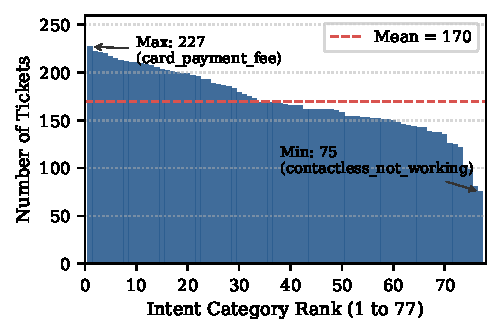
\includegraphics[width=\columnwidth]{figures/intent_distribution.pdf}
\caption{Intent distribution across all 77 categories in the BANKING77 dataset ranked by frequency ($\mu = 170$, range $75$ to $227$).}
\label{fig:intent_dist}
\end{figure}

\begin{figure}[!tb]
\centering
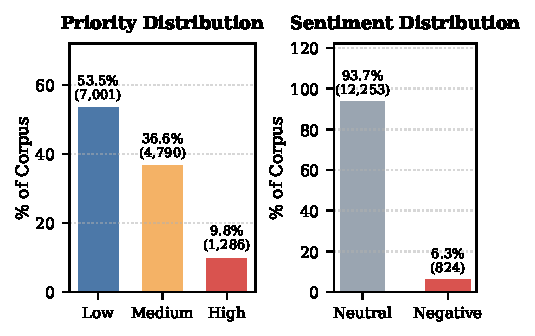
\includegraphics[width=\columnwidth]{figures/task_imbalance.pdf}
\caption{Operational class imbalance across Priority tiers (left) and Sentiment targets (right) over the 13{,}077 ticket corpus.}
\label{fig:task_imbalance}
\end{figure}

As shown in Fig.~\ref{fig:intent_dist}, BANKING77 intents display balanced coverage across all 77 categories ($\mu = 169.8$ tickets, range $75$ to $227$, normalized entropy 0.982). In contrast, the resulting operational targets exhibit severe class imbalance (Fig.~\ref{fig:task_imbalance}): Priority follows an inverse severity distribution with 53.5\% Low, 36.6\% Medium, and only 9.8\% High urgent tickets. Sentiment is 93.7\% Neutral and 6.3\% Negative, capturing customer dissatisfaction and distress for queue escalation.
